Successful implementation of {\IT} will serve three communities, including two types of researchers along with software engineering practitioners. 
First, {\IT} will provide an infrastructure to allow researchers to gain a better understanding of a broad range of topics across \textit{General Software Engineering Research}.
Second, {\IT} will provide a platform where \textbf{Empirical Software Engineering and Text Mining Researchers} can experiment with different techniques and workflows to identify the most effective approaches.
Finally, {\IT} will enable \textbf{Software Engineering Practitioners} to benefit from the synthesized research results.
Figure~\ref{figure-ResearchEnabled} provides an overview of these communities.

\begin{figure}
	\centering
	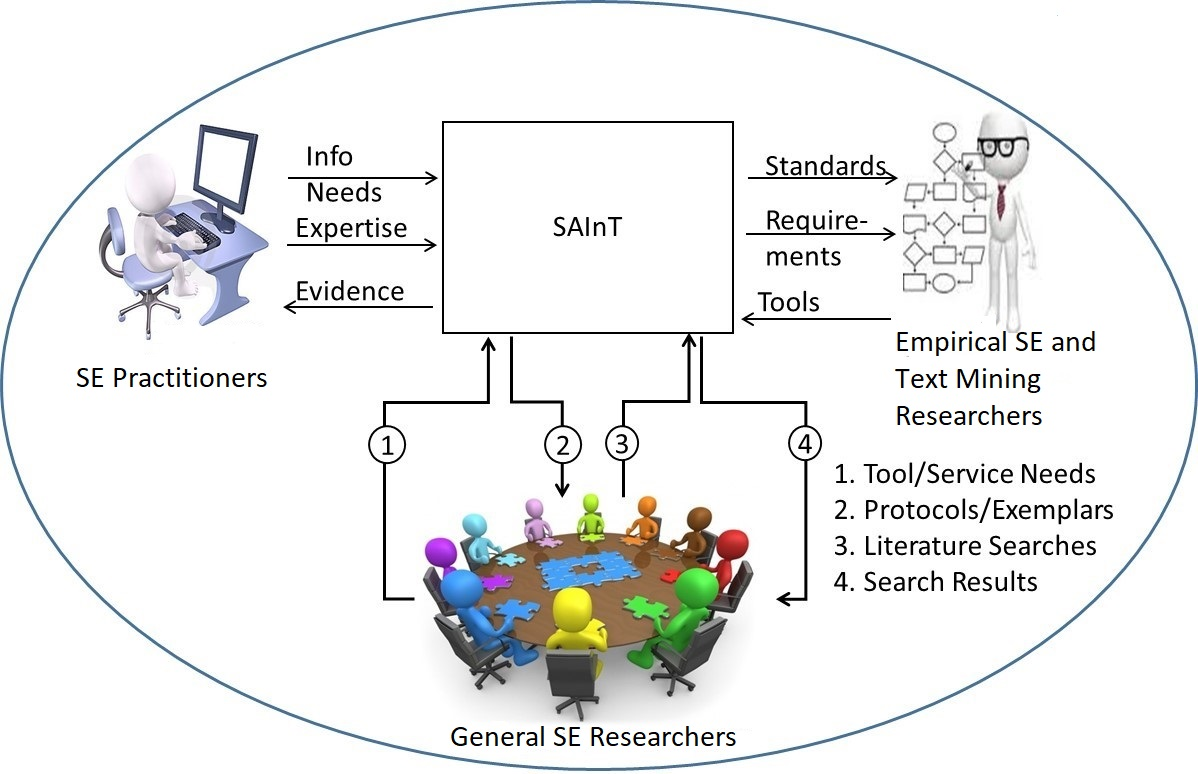
\includegraphics[width=4.5in]{ResearchEnabled}
	\caption{Research Enabled}
	\label{figure-ResearchEnabled}
\end{figure}

\vspace{8pt}
 
%Before committing to {\IT} as a solution technology, it is appropriate  to ask what problem does it actually solve?  That is to say, if  {\IT} is the answer, what CISE question does it address?
% Given all the recent changes in software engineering\footnote{The end of the waterfall era. 
% 	The rise of agile and devops. Internationalization of software development.
% 	Distributed software development. 
% 	Cloud environments. 
% 	A large number of next-generation computer languages. 
% 	A larger number of programmers writing more programs. Application of AI to SE.}
% it is high time to update established wisdom. 
% Because much of that wisdom was first recorded decades ago, it is an open question as to which prior claims need to be updated. 
% The following are examples of conclusions that contradict prior work:
% \bi
% \item Strongly typed languages are not necessarily associated with more successful projects~\cite{ray2014large};  
% \item
% The language construct GOTO, as used in contemporary practice, is rarely
% considered harmful~\cite{nagappan2015empirical};
% \item Test-driven development may not be  any better than "test last"~\cite{fucci2017dissection};
% \item Delayed issues are rarely exponentially more expensive to fix~\cite{menzies2017delayed};
% \item In stark contrast to  much prior research, pre- and post- release failures are not connected~\cite{fenton2000quantitative};
% \item Static code analyzers perform no better than simple statistical predictors~\cite{Fa13}.
% \ei

% That is, one reason to augment standard SLRs with AI tools (as done in {\IT}) is that the SE field urgently  needs to rethink its core premises using more of the current evidence.
% This rethinking is important not only for researchers, but also for practitioners.
% Among developers, there is frequently little agreement on what many factors most effect software projects:
% \bi
% \item According to Passos et al.,  developers often assume that the lessons they learn from a few past projects are general to all their future projects. 
% They comment, ``past experiences were taken into account without much consideration for their context''~\cite{Pa11}. 
% \item J{\o}rgensen \& Gruschke offer a similar warning. 
% They report that the supposed software engineering ``gurus'' rarely use lessons from past projects to improve their future reasoning and that such poor past advice can be detrimental to new projects~\cite{Jo09}.
% \item Other studies have shown some widely-held views are now questionable given new evidence.
% 	Devanbu et al. examined responses from 564 Microsoft software developers from around
% 	the world. 
% 	They comment programmer beliefs can vary with each project, but do not necessarily correspond with actual evidence in that project~\cite{De16}. 
% \ei
% \begin{table*}[!b]
%   \centering
%   \caption{A hierarchy of evidence for software engineering research. From the {\SHAW} paper~\cite{Goues18}.
%  }\label{tbl:evidence}
%  {\small
%   \begin{tabular}{|p{1cm}|p{2cm}|c|p{10.5cm}|}
%     \rowcolor{gray} \multicolumn{2}{|l|}{\textcolor{white}{Type of study}}&\textcolor{white}{Level} &\textcolor{white}{Evidence}   \\\hline
     
%     \multicolumn{2}{|l|}{Secondary or filtered studies} & 0 & Systematic reviews with recommendations for practice; meta-analyses\\
%     \hline
%      & {Systematic  } & 1 & Formal or analytic results with rigorous derivation and proof \\
%     \cline{3-4}
%       &&2&Quantitative empirical studies with careful experimental design and good statistical control\\
%     \cline{2-4}
     
%     &{Observational  } & 3 & Observational results supported by sound qualitative methods, including well-designed case studies\\
%     \cline{3-4} 
%   Primary &&4&Surveys with good sampling + good design; field studies; data mining\\
%     \cline{3-4}
%   studies &&5&Experience from multiple projects, with analysis and cross-project comparison; a tool, a prototype, a notation, a dataset, or another artifact (that has been certified as usable by others)\\
%     \cline{3-4} 
%     &&6&Experience from a single project: an objective review of a specific project; lessons learned; a solution to a specific problem, tested and validated in the context of that problem; an in-depth experience report; a notation, a dataset, or an unvalidated artifact\\
%     \hline 
%     \multicolumn{2}{|l|}{No design} & 7 & Anecdotes on practice; a rule of thumb; an evaluation with small or toy examples; a novel idea backed by strong argumentation; a position paper or an op-ed based principally on expert opinion\\\hline
%   \end{tabular}}
% \end{table*}

% The {\SHAW} paper  note that the above are a symptoms of a researcher
%   community that is poorly defining its research outputs. They say:
%   \begin{quote}
%   {\em When engineers seek answers to their practical problems, ``perfect'' scientific knowledge is not always available. If it's not, engineers readily accept ``good-enough'' evidence: case studies, small-scale experiments, blog posts, or even advice from acknowledged experts.}~\cite{Goues18} 
%   \end{quote}
% Their challenge to the community is to provide better ``good-enough'' evidence. In this proposal,
% we explore the application of AI tools to text mining to provide such good enough evidence.

\paragraph{General Software Engineering Researchers}

\vspace{8pt}
\paragraph{Empirical Software Engineering and Text Mining Researchers}
We also plan to support these researchers by providing a platform to experiment  with  different techniques  and  workflows. Empirical software engineering researchers have established some recommended workflows (e.g. pilot search and keyword refinement) and strategies (e.g. snowballing~\cite{jalali2012systematic}) to improve the efficiency and quality of SLRs. Meanwhile, many text mining researchers have selected SLRs as case studies to test the effectiveness of different machine learning algorithms (e.g. active learning~\cite{Yu2018} and visual text mining~\cite{Felizardo2010An}). {\IT} as a platform will facilitate the testing of mix-and-matching different workflows, strategies, and algorithms, thus benefit the research of both empirical software engineering and text mining. It will also be beneficial to have {\IT} as a testbed for the latest developed algorithms from text mining and machine learning, e.g. word2vec, deep neural networks, named entity recognition, part-of-speech tagging, etc.

\vspace{8pt}
\paragraph{Software Engineering Practitioners}
In addition to the benefits to researchers described above, the numerous consumers that utilize the results of SLRs will also benefit from the work.  
Practitioners and executives in industry utilize SLR results to identify best practices and to guide decision making.  
Industrial software engineers will benefit from more applied and relevant research that they can commission.
Other researchers have already begun building methods (e.g. Visual Abstracts~\cite{VisualAbstracts}) for representing the findings of SLRs in a format that is useful to practitioners.
By helping researchers produce more SLRs that represent all of the literature, {\IT} will help the results presented to industry be more complete and accurate.

\vspace{8pt}
% offering such 
% {\SHAW} remarks:
% \begin{quote}
% {\em We envision a system that allows researchers and practitioners to reliably synthesize research results into actionable, real-world guidance.  We are proposing not a new sub-field of SE but rather a new way to label, organize, and synthesize results across SE to more concretely benefit practice. This vision is achievable, given sufficient community participation and cooperation.}~\cite{Goues18} 
% \end{quote}
% The {\SHAW} paper is more of a  ``vision'' document than a list of technical details
% on how to proceed. But they do offer the following guidelines on how to index SE research results in a ``good-enough'' manner. They say their preferred tool set required
% the following:
% \begin{itemize}[  leftmargin=+.5in, itemsep=0pt, parsep=0pt]
% \item[7a:]
%  Explicit identification of methods and results.
% %We note that this is a {\em classification} and
% %{\em entity extraction} problem that could be automated with AI tools. That is, while it is certainly best
% %if authors self-identify the methods and results within their papers, it is possible for AI tools to at least propose what methods and results might be %within a paper (which a human could then confirm or reject).
% \item[7b:]
% Consensus on a formal framework for 
% {\em levels of evidence}, together with a mapping between the evidence and the strength of the resulting recommendation. 
% \item[7c:]
% Incentives for and recognition of reviews that synthesize, interpret, or provide meta-analysis of bodies of prior work. 
% \item[7d:]
%  Education of software engineers in how to use the framework.  
% \end{itemize}
%  We will return to this list, later in this proposal, when we discuss the ``{\SHAW} factor''; i.e. how well does {\IT} addresses the challenges set out in the {\SHAW} paper.